\documentclass[10pt,aspectratio=169]{beamer}
\usetheme{Madrid}
\usecolortheme{seahorse}
\useinnertheme{circles}
\setbeamertemplate{navigation symbols}{}
\setbeamertemplate{caption}{\insertcaption}
\usepackage[T1]{fontenc}
\usepackage{lmodern}
\usepackage{amsmath,amssymb}
\usepackage{booktabs}
\usepackage{multirow}
\usepackage{graphicx}

\newcommand{\hl}[1]{\textcolor{blue!60!black}{\textbf{#1}}}

\title[Deriving \& Bounding the Multi-Power Law]{Deriving, Testing, and Bounding the Multi-Power Law\\for Schedule-Aware Loss-Curve Prediction}
\author[Jiaju Wu]{Jiaju Wu \quad (2400010711, Undergraduate)}
\institute[]{Deep Learning --- Task 2 \quad\textbar\quad \texttt{github.com/wjjpku/DL-final}}
\date{}

\begin{document}

{\setbeamertemplate{footline}{}
\begin{frame}\titlepage
\small
\textbf{One-line summary:} we reproduce the two empirical loss-curve laws (Tissue,
MPL), \emph{derive} MPL from SGD dynamics (a discrete cousin of the kernel-regression
functional scaling law of Li et al.\ 2025), confirm its predicted scale-invariance
(all 27 curves collapse onto one master curve, $R^2{=}0.997$), try \emph{four}
principled ways to \emph{beat} it (honest result: MPL is near-optimal), and give its
one empirical parameter $\gamma$ a corrected \emph{edge-of-stability} origin
(river-valley sharpening lag) while showing it is near-irreducible.
\vfill
{\footnotesize\itshape These slides are written as a \textbf{self-contained report}:
each slide states its setup, its result, and a boxed/bold \textbf{takeaway}, so they
can be read without an oral presentation. Every number is reproduced by a named
script (final two slides).}
\end{frame}}

\begin{frame}{Outline}
\tableofcontents
\end{frame}

% =====================================================================
\section{Problem \& Motivation}
\begin{frame}{The problem: schedule-aware loss-curve prediction}
\textbf{Goal.} Given a learning-rate (LR) schedule $\{\eta_t\}$, predict the whole
pretraining loss curve $L(t)$ \emph{before} running the training.
\vfill
\textbf{Why it matters.}
\begin{itemize}
  \item Pretraining LLMs is expensive; the LR schedule strongly shapes the entire
  loss trajectory, not just the endpoint.
  \item Classical scaling laws (Kaplan, Chinchilla) predict only the \emph{final}
  loss vs.\ model size / data --- they say nothing about the curve's response to
  the schedule \emph{shape} (warmup, decay form, horizon).
  \item A good law (i) replaces trial runs with a formula, (ii) exposes
  mid-training dynamics (the extra drop from LR decay), and (iii) can be inverted
  to \emph{search} for better schedules.
\end{itemize}
\vfill
\textbf{The defining test --- cross-schedule generalization:}
\hl{fit on cosine schedules, predict the unseen WSD family.}
\end{frame}

\begin{frame}{What this project does}
We go beyond reproduction and study the governing law itself:
\begin{enumerate}
  \item[\textbf{1.}] \textbf{Reproduce} the two representative laws (Tissue 2024;
  Multi-Power Law / MPL, Luo 2025) on the cosine$\to$WSD task.
  \item[\textbf{2.}] \textbf{Derive} MPL's functional form from SGD on a power-law
  curvature spectrum --- giving each parameter a physical meaning and a prediction.
  \item[\textbf{3.}] \textbf{Test} the prediction: kernel exponents are
  scale-invariant $\Rightarrow$ all curves collapse onto one master curve.
  \item[\textbf{4.}] \textbf{Improve?} Four principled methods (SC-MPL; a new
  $(S,Q)$ asymptotic; an explicit river-valley law; a sharpness-lag correction) ---
  honest finding: MPL is near-optimal here.
  \item[\textbf{5.}] \textbf{Bound:} give MPL's one empirical parameter $\gamma$ a
  corrected \emph{edge-of-stability} origin and show it is near-irreducible.
\end{enumerate}
\vfill
\centering\footnotesize
Data: official public loss curves, $3$ scales ($25/100/400$M) $\times\ 9$ schedules.
\end{frame}

% =====================================================================
\section{Background \& Reproduction}
\begin{frame}{Background: the two empirical laws}
Let $S(t)=\sum_{i\le t}\eta_i$ be the \hl{cumulative LR} (a natural ``time''), and
$\Delta\eta_k=\eta_{k-1}-\eta_k$ the LR decrement at step $k$.
\vfill
\textbf{Tissue et al.\ (5 parameters)} --- simple, interpretable, but coarse:
\[ L(t)=L_0+A\,S(t)^{-\alpha}-C\,S_2(t),\qquad S_2=\text{momentum-smoothed annealing area.}\]
\textbf{Multi-Power Law / MPL (7 parameters)} --- current state of the art:
\[ L(t)=L_0+\underbrace{A\,S(t)^{-\alpha}}_{\text{backbone}}+B\!\!\underbrace{\sum_{k\le t}\!\Delta\eta_k\,G\!\big(\eta_k^{-\gamma}(S(t)-S(k))\big)}_{\text{loss-drop term }LD},\quad G(x)=1-(1+Cx)^{-\beta}.\]
\vfill
\textbf{How to read MPL.} The \emph{backbone} $A\,S^{-\alpha}$ is the loss you would
get at the current cumulative LR with no decay. The \emph{loss-drop} term $LD$ adds
the bonus from every past LR decrease $\Delta\eta_k$: $G$ is a \hl{saturating} kernel
(rises $0\!\to\!1$), so each decrement's benefit accrues over ``time'' $S(t)-S(k)$
and then plateaus. The factor $\eta_k^{-\gamma}$ rescales that time by the LR at which
the decrement happened --- it is \hl{fit empirically}, with no derivation in the
original paper. \emph{Pinning down this $\gamma$ is the through-line of this project.}
\end{frame}

\begin{frame}{Reproduction: setup}
\textbf{Setup (following the task).}
\begin{itemize}
  \item Data: official MPL loss curves, $25/100/400$M, $9$ schedules each.
  \item \hl{Fit on cosine} schedules (\texttt{cosine\_24000}, \texttt{cosine\_72000});
  \hl{evaluate on $5$ unseen WSD curves} (\texttt{wsd}, \texttt{wsdld},
  \texttt{wsdcon\_\{3,9,18\}}).
  \item Objective: Huber loss on $\log L$; optimizer: L-BFGS-B with multi-start.
  \item Engineering: Tissue's $S_2$ rewritten as an exact linear recurrence
  ($\sim\!100\times$ faster); MPL's $LD$ vectorized.
\end{itemize}
\vfill
\textbf{Metric.} Average test MAE over the $5$ WSD curves (lower is better).
\vfill
\footnotesize Code: \texttt{repro/reproduce\_cosine\_to\_wsd.py}.
\end{frame}

\begin{frame}{Reproduction: results match the published numbers}
\begin{columns}
\begin{column}{0.46\textwidth}
\centering
\begin{table}\small
\begin{tabular}{lcc}
\toprule
Scale & Tissue (5p) & MPL (7p) \\
\midrule
25M  & 0.00783 & \textbf{0.00539}\\
100M & \textbf{0.00486} & 0.00496\\
400M & 0.00979 & \textbf{0.00852}\\
\bottomrule
\end{tabular}
\end{table}
\vspace{0.5em}
{\footnotesize avg test MAE on WSD (fit on cosine)}
\end{column}
\begin{column}{0.54\textwidth}
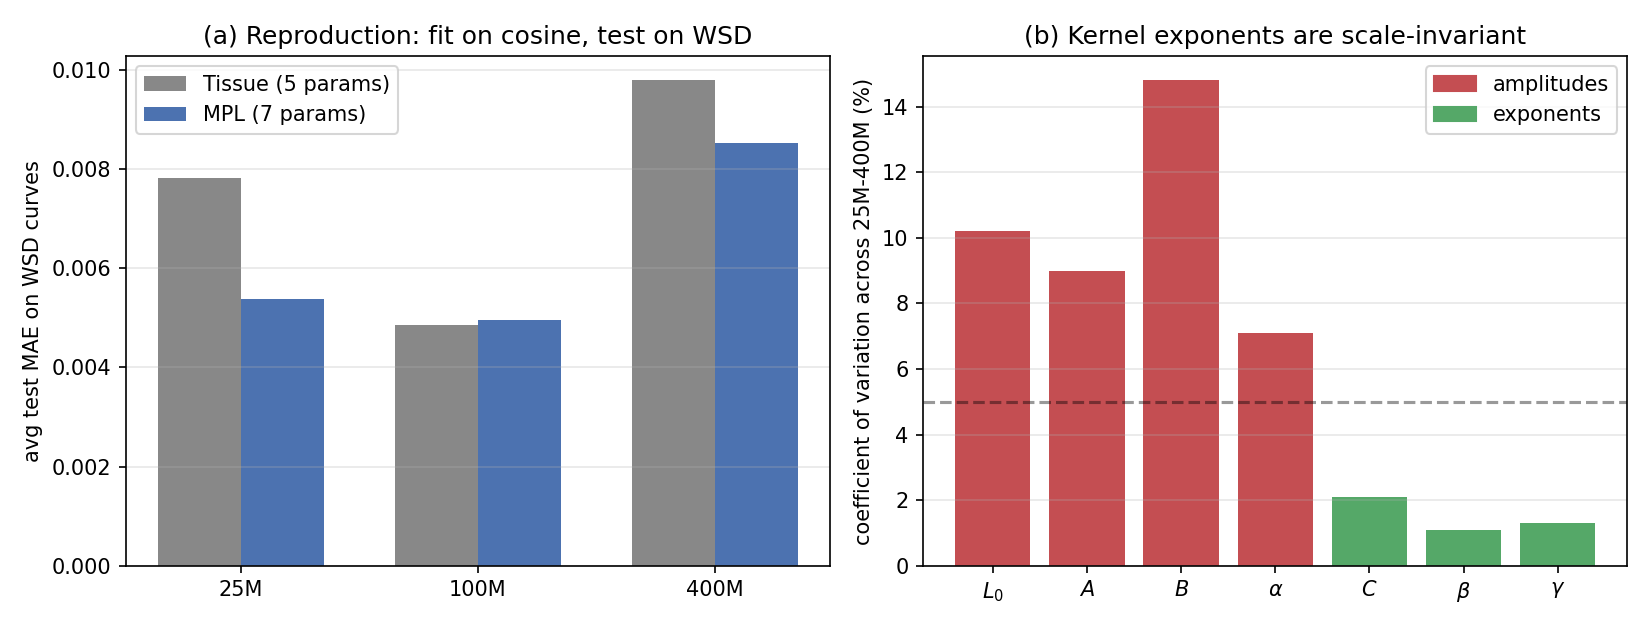
\includegraphics[width=\linewidth]{figs/fig1_repro_invariance.png}\\
{\footnotesize\textit{Fig.\ 1(a): predicted curves (lines) vs.\ ground-truth loss
(dots) on held-out WSD schedules; closer is better.}}
\end{column}
\end{columns}
\vfill
\textbf{Analysis (what the numbers say).} We recover the published behavior: MPL is
more accurate at $25/400$M and ties Tissue at $100$M, and generalizes more stably
across schedule shapes. Our MPL test MAE ($0.0054/0.0050/0.0085$ at $25/100/400$M)
matches Luo et al., confirming the reproduction is faithful.
\hl{This well-fit MPL is the baseline the rest of the work must respect} --- every
later ``improvement'' is measured against a properly-optimised MPL, not a weak one.
\end{frame}

% =====================================================================
\section{Deriving MPL from SGD Dynamics}
\begin{frame}{Why derive it? From 7 opaque parameters to physical meaning}
\textbf{Goal of this section.} MPL fits well but its 7 parameters are a black box.
We derive its \emph{form} from a simple dynamical model so each parameter gets a
physical identity \emph{and} a testable prediction about how it scales with model size.
\vfill
\textbf{Model.} Near the trajectory the loss is locally quadratic. In the Hessian
eigenbasis, mode $i$ has curvature $\lambda_i$ and gradient-noise variance
$\sigma_i^2$; $\delta_i(t)$ is the distance to the optimum along that mode, and one
SGD step is the linear noisy recurrence
\[ \delta_i(t{+}1)=(1-\eta_t\lambda_i)\,\delta_i(t)-\eta_t\xi_i(t),\qquad
L=L_{\min}+\tfrac12\textstyle\sum_i\lambda_i\,\mathbb E[\delta_i^2].\]
Each step shrinks mode $i$ by $(1-\eta_t\lambda_i)$ and injects noise. The mean
square $\mathbb E[\delta_i^2]$ splits into a \hl{bias} (deterministic shrinkage of
the initial gap) and a stochastic \hl{noise floor}.
\vfill
\textbf{(1) Bias $\to$ power-law backbone.} The bias shrinks as
$\delta^{\text{bias}}\!\approx\!\delta(0)\,e^{-\lambda S}$, governed by the
\hl{cumulative LR} $S(t)=\sum_{i\le t}\eta_i$ (high-curvature modes die first; flat
modes persist). Summing over a power-law density of curvatures
$g(\lambda)\sim\lambda^{a}$, a Tauberian (Laplace-transform) argument turns the
mixture of exponentials into a single power law:
\[ L_{\text{bias}}(S)=\!\int_0^\infty\! g(\lambda)\,e^{-2\lambda S}\,d\lambda \;\sim\; A\,S^{-\alpha},
\quad \alpha=a+1,\quad L_0=L_{\min}.\]
\centering\hl{Takeaway:} the $A\,S^{-\alpha}$ backbone is just ``many modes relaxing
at a power-law spread of rates.''
\end{frame}

\begin{frame}{The annealing term and a falsifiable prediction}
\textbf{(2) Noise floor $\to$ annealing term.} The stochastic part obeys
$V_i(t)\!\approx\!\sigma_i^2\!\int_0^{S(t)}\!\eta(S')\,e^{-2\lambda_i(S(t)-S')}dS'$:
the iterate carries a cloud of noise whose size tracks the \emph{current} LR, so at
constant LR the noise loss is $\propto\eta$ (\hl{the floor tracks the current LR}).
When the LR \emph{decays}, this floor shrinks --- that extra drop, written as a sum
over the per-step LR \emph{decrements} $\Delta\eta_k$, is
\[ \Delta N(t)=\sum_k \Delta\eta_k\,\mathcal{K}\!\big(S(t)-S(k)\big)\quad\text{--- this is \emph{exactly} MPL's loss-drop term }LD.\]
Assuming a \hl{Gamma-shaped} curvature spectrum
$\propto\lambda^{\beta-1}e^{-\lambda/\lambda_0}$ makes the kernel
$\mathcal{K}(y)\propto 1-(1+Cy)^{-\beta}$ with $C=2\lambda_0$ --- \emph{precisely}
MPL's $G$. So the whole form of MPL (backbone $+$ $LD$) drops out of the dynamics.
\vfill
\textbf{Each parameter now has an identity:}
\begin{center}\small
\begin{tabular}{ll}
\hl{Exponents} $\{\alpha,\beta,C\}$ & = functions of the spectral \emph{shape} (the density's exponents)\\
\hl{Amplitudes} $\{L_0,A,B\}$ & = set by the irreducible loss + spectral \emph{scale}\\
\end{tabular}
\end{center}
\textbf{Falsifiable prediction.} If the curvature spectrum keeps its \emph{shape} as
model size $N$ grows (only its scale changes), then the \hl{exponents must be
scale-invariant} and only the amplitudes drift with $N$. We test this next.
\end{frame}

\begin{frame}{Where this sits: theory, empirics, and learned laws}
Our SGD--spectrum derivation is a \hl{discrete-spectrum cousin} of the
kernel-regression theory of \hl{Li, Chen, Huang, Wang \& Wu (2025)},
\emph{Functional Scaling Laws} (FSL, NeurIPS'25):
\begin{center}\small
\begin{tabular}{lll}
\toprule
 & FSL (Li et al.\ 2025) & this work \\
\midrule
model            & SGD on power-law kernel regression & SGD on power-law Hessian spectrum\\
``time''         & intrinsic time & cumulative LR $S(t)=\sum\eta_i$\\
schedule enters via & a convolutional functional & the decrement kernel $LD$\\
instantiated on  & const / exp-decay / WSD (theory) & real MPL curves, $25/100/400$M\\
\bottomrule
\end{tabular}
\end{center}
\vfill
\textbf{The landscape of laws.} \emph{Tissue} (momentum law) and \emph{MPL}
(empirical) are closed forms; \emph{FSL} is the matching kernel-regression theory;
\emph{NCPL} (Zhang, Wen \& Ma 2026) instead \hl{learns} a neural configuration
$\to$ performance map (evaluated on the StepLaw dataset). \hl{We take the
interpretable closed-form route}: derive MPL, confirm its universality, and pin
down its one irreducible parameter.
\end{frame}

% =====================================================================
\section{Scale Invariance \& a Universal Master Curve}
\begin{frame}{Result 1: the kernel exponents are scale-invariant}
\begin{columns}
\begin{column}{0.5\textwidth}
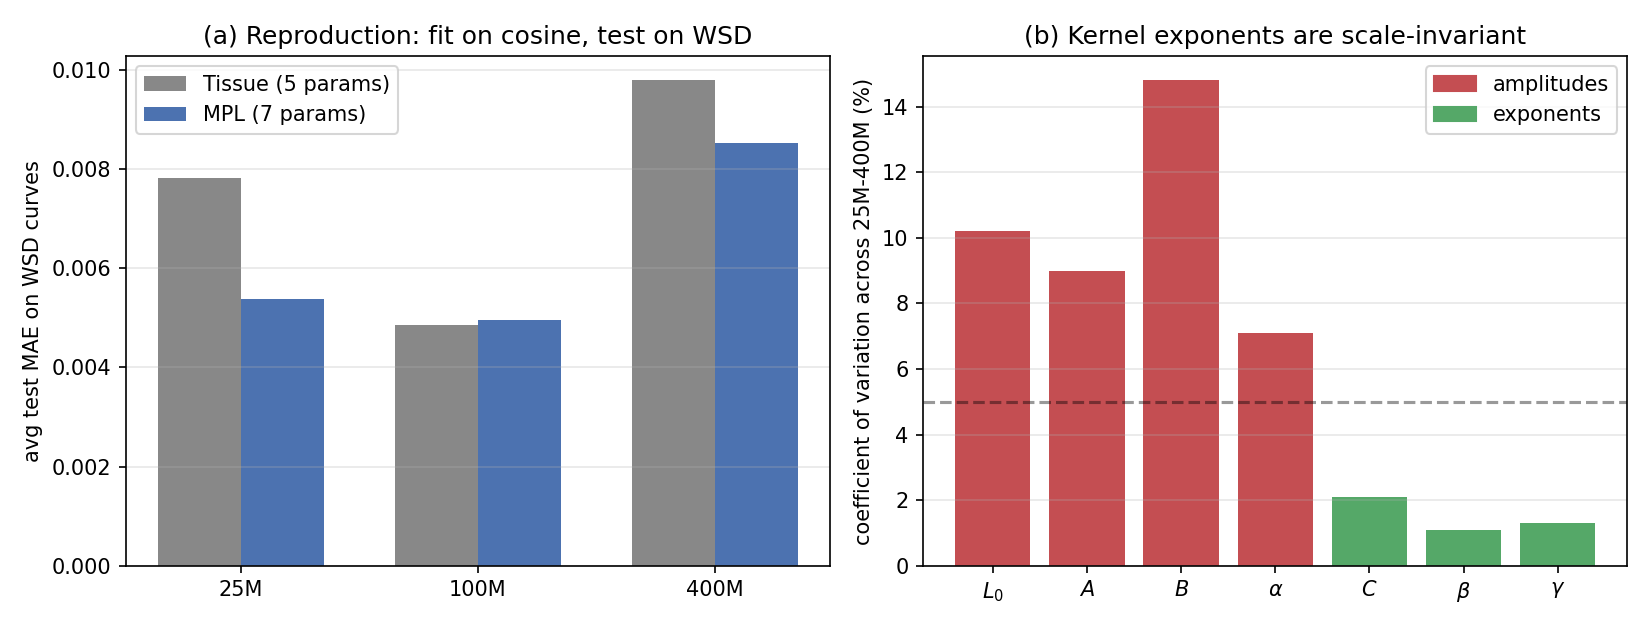
\includegraphics[width=\linewidth]{figs/fig1_repro_invariance.png}\\
{\footnotesize\textit{Fig.\ 1(b): each fitted parameter vs.\ model size. The
exponent curves are flat; the amplitude curves are sloped.}}
\end{column}
\begin{column}{0.5\textwidth}
Fitting MPL separately at each scale and comparing parameters across a \hl{$16\times$}
size range ($25\!\to\!400$M):
\begin{itemize}
  \item Exponents $C,\beta,\gamma$: CV $=\,$\hl{$2.1\%,\,1.1\%,\,1.3\%$} (essentially constant).
  \item Amplitudes $L_0,A,B$: CV $=9\text{--}15\%$ (drift with $N$).
  \item $\alpha$ (initialization-weighted, predicted least stable of the exponents): $7\%$.
\end{itemize}
\vspace{0.4em}
\hl{The prediction is confirmed:} the shape of the annealing response is a near
scale-invariant constant; only the amplitudes carry the size dependence.
\end{column}
\end{columns}
\end{frame}

\begin{frame}{Result 2: all 27 curves collapse onto one master curve}
\begin{columns}
\begin{column}{0.56\textwidth}
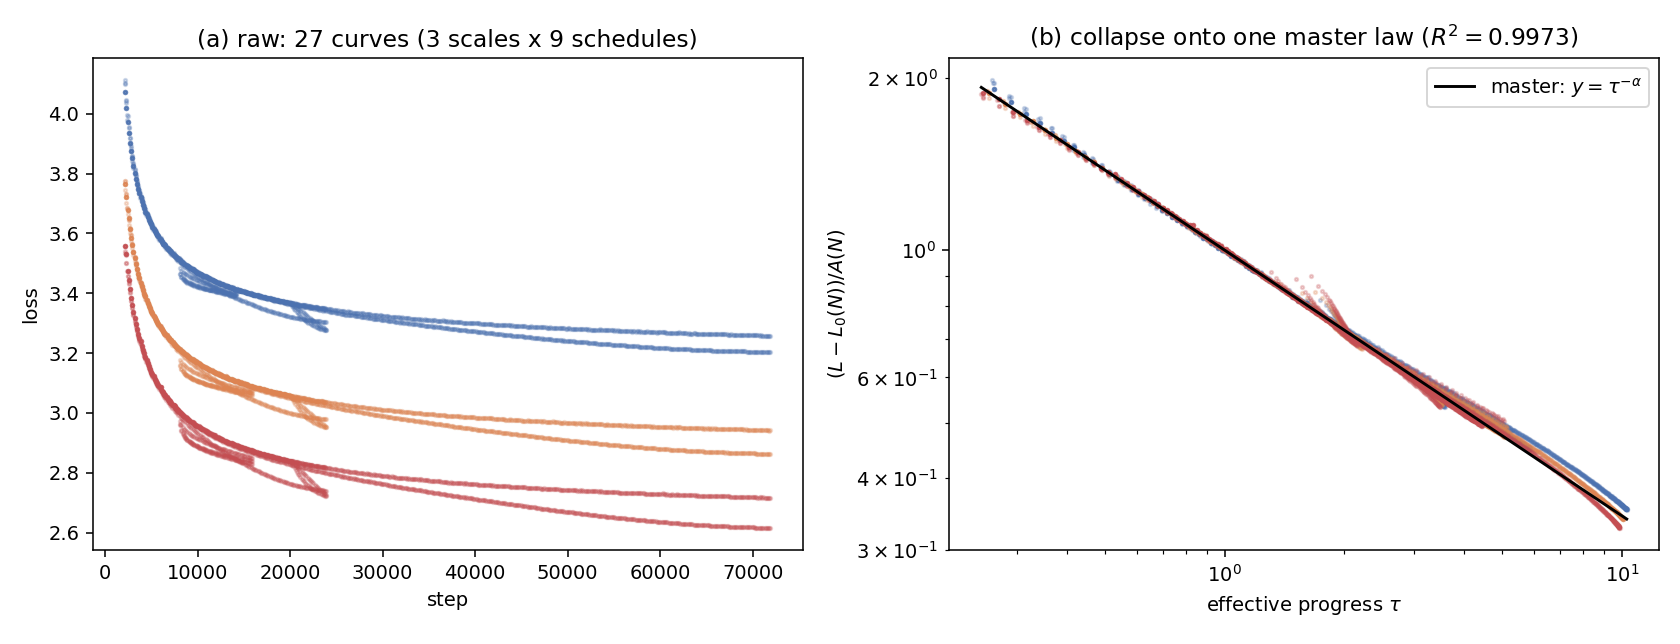
\includegraphics[width=\linewidth]{figs/fig2_collapse.png}\\
{\footnotesize\textit{Top: 27 raw loss curves (3 sizes $\times$ 9 schedules).
Bottom: after the $\tau$-rescaling they fall on one line $y=\tau^{-\alpha}$.}}
\end{column}
\begin{column}{0.44\textwidth}
Rearranging MPL algebraically shows it is really a \emph{single} power law
$L=L_0(N)+A(N)\,\tau^{-\alpha}$ in one \hl{effective-progress} variable
\[ \tau=\big[\,S^{-\alpha}+(B/A)\,LD\,\big]^{-1/\alpha},\]
which absorbs the entire schedule (backbone $+$ annealing) into a single number per
step --- ``how far along the universal curve are we.''
\vspace{0.4em}

Using \hl{one shared exponent set} for all scales and only per-scale amplitudes, all
\hl{$27$ curves} collapse onto $y=\tau^{-\alpha}$ with \hl{$R^2=0.997$}.
\end{column}
\end{columns}
\vfill
\textbf{Analysis.} The collapse succeeds \emph{only because a single exponent set
fits every scale} --- a direct visual proof of scale invariance. There is
essentially \hl{one} loss curve; model size and schedule merely reparameterize the
axes. \hfill{\footnotesize Code: \texttt{repro/universal\_collapse.py}}
\end{frame}

% =====================================================================
\section{Method Development: Can We Improve MPL?}
\begin{frame}{Attempt 1 --- SC-MPL: a scale-conditioned law}
\textbf{Idea.} Since the exponents are scale-invariant, \hl{borrow them from cheap
small models} and fit only the $3$ amplitudes $\{L_0,A,B\}$ on the target scale ---
cutting a new scale from $7$ free parameters to $3$.
\vfill
\begin{columns}
\begin{column}{0.5\textwidth}
\centering\small
\begin{tabular}{lccc}
\toprule
Scale & MPL & SC-4 & SC-3 \\
\midrule
100M & \textbf{0.00435} & 0.00451 & 0.00525\\
400M & \textbf{0.00484} & 0.00760 & 0.00786\\
\bottomrule
\end{tabular}\\[2pt]
{\footnotesize fair comparison, official split, avg test MAE}
\end{column}
\begin{column}{0.5\textwidth}
\textbf{Honest result.} Competitive at $100$M (wins $4/6$ curves with far fewer
parameters) but \hl{does not beat a well-fit MPL at $400$M}: the residual drift
(chiefly in $\alpha$) costs more than the parameter economy gains.
\end{column}
\end{columns}
\vfill
\textbf{A methodological caution we discovered.} An earlier protocol that
\emph{re-fit} the MPL baseline into a poor optimum made SC-MPL look $20\%$ better;
giving the baseline its \hl{true} optimum erases that ``win.''
\emph{An under-optimized baseline can fabricate a false result.}
\end{frame}

\begin{frame}{Attempt 2 --- Q-MPL: a new discrete-step asymptotic}
\textbf{New angle.} Tissue and MPL both use the continuum approximation, leaving
the single time variable $S=\sum\eta$. Keeping the \hl{next discrete-step order}
introduces a \emph{second} time variable:
\[ \textstyle\prod(1-\eta\lambda)^2\approx e^{-2\lambda S-\lambda^2 Q},\qquad Q=\sum\eta^2.\]
Expanding the bias integral yields a \hl{derived correction} $\propto Q\,S^{-(\alpha+2)}$.
We test $\;\text{Q-MPL}=\text{MPL}+E\cdot Q\,S^{-(\alpha+2)}\;$ ($8$ params).
\vfill
\begin{columns}
\begin{column}{0.46\textwidth}
\centering\small
\begin{tabular}{lccc}
\toprule
Scale & MPL & Q-MPL & $E^\ast$\\
\midrule
25M  & \textbf{0.00715} & 0.00715 & ${\approx}0$\\
100M & \textbf{0.00386} & 0.00386 & ${\approx}0$\\
400M & \textbf{0.00669} & 0.00824 & overfit\\
\bottomrule
\end{tabular}
\end{column}
\begin{column}{0.54\textwidth}
\textbf{Honest result.} The data drive $E\!\to\!0$ at $25/100$M (the term is
unnecessary), and when free it \hl{over-fits cosine and worsens WSD} at $400$M.
\hl{Q-MPL does not beat MPL.}
\end{column}
\end{columns}
\end{frame}

\begin{frame}{Verdict: MPL is near-optimal on the current data}
Two \emph{principled} extensions --- scale-conditioning and a new $(S,Q)$
asymptotic --- both fail to improve a well-fit MPL (two more, built on the
edge-of-stability mechanism, follow in \S6 and also fail). The universal collapse
($R^2{\approx}0.997$) shows MPL already captures essentially all reproducible
structure.
\vfill
\begin{block}{Honest conclusion}
On these curves MPL is near-optimal: the residual ($\text{MAE}\!\sim\!0.003$)
carries no structure that a derived correction exploits.
\end{block}
\vfill
\textbf{Why, and what would change it.} MPL was developed and tuned on exactly this
kind of (relatively mild) data. Beating it would likely require data that
\hl{exposes MPL's failure modes} --- more extreme schedules or more model scales ---
which is the natural data bottleneck of this study.
\end{frame}

% =====================================================================
\section{The Edge-of-Stability Origin of $\gamma$}
\begin{frame}{MPL's one empirical parameter: $\gamma$ is essential, but not from theory}
The factor $\eta_k^{-\gamma}$ is the only part of MPL our derivation does
\emph{not} produce. Is it actually needed?
\vfill
\begin{columns}
\begin{column}{0.4\textwidth}
\centering\small
\begin{tabular}{lcc}
\toprule
Scale & full MPL & $\gamma{=}0$\\
\midrule
25M  & 0.0032 & 0.0119\\
100M & 0.0038 & 0.0144\\
400M & 0.0049 & 0.0162\\
\bottomrule
\end{tabular}\\[2pt]
{\footnotesize real data, test MAE}
\end{column}
\begin{column}{0.6\textwidth}
Setting $\gamma{=}0$ (re-fitting amplitudes) makes the prediction \hl{$3\text{--}4\times$
worse} --- so $\gamma$ is \hl{essential}.
\vspace{0.4em}

Yet it \emph{cannot} come from the spectral theory: in $S$-units the leading kernel
has no $\eta$ factor, so the model predicts $\gamma{=}0$, and a quadratic-SGD
\hl{simulation confirms} a $\gamma{=}0$ kernel fits the simulated curves as well as
full MPL. So $\gamma$ lives \emph{outside} the quadratic picture. Where?
\end{column}
\end{columns}
\end{frame}

\begin{frame}{The corrected origin: an \emph{adaptive} river valley}
\textbf{Fixing a common misconception.} The data are trained with \hl{AdamW}, not
gradient descent --- so the operative edge is \emph{not} sharpness$\,{=}\,2/\eta$,
but the \hl{adaptive edge of stability} (Cohen et al.\ 2022). AdamW pretraining
traverses a \hl{river-valley} landscape (Wen et al.\ 2024): a flat ``river''
(progress) and sharp ``mountain'' directions (oscillation).
\vfill
For a mountain mode of curvature $H$, the stationary excess loss of discrete SGD is
\emph{exactly}
\[ P_{\rm osc}(\eta,H)=\frac{\sigma^2}{2}\,\frac{\eta}{2-\eta H}. \]
\begin{itemize}\small
  \item $\eta H\!\to\!2$ (the edge) $\Rightarrow P_{\rm osc}\!\to\!\infty$: the
  \hl{elevated stable-phase loss}.
  \item $\eta\!\to\!0$ (decay) $\Rightarrow P_{\rm osc}\!\to\!0$: the decay
  \hl{``reveals'' accumulated progress}.
  \item $H$ is a \hl{lagging state} (progressive sharpening, timescale $\tau$). If
  $H$ tracked $\eta$ instantly, $P_{\rm osc}\!\propto\!\eta$ and \emph{no} $\gamma$
  is needed; a finite lag after a \hl{sharp} decay makes the penalty
  history-dependent --- exactly what $\eta_k^{-\gamma}$ encodes.
\end{itemize}
\vspace{0.3em}
\centering\hl{$\gamma$ = the effective exponent of the sharpening lag.}
\end{frame}

\begin{frame}{Two explicit laws --- and why $\gamma$ is near-irreducible}
We replaced $\gamma$ by the mechanism itself (theory first, then experiment):
\begin{columns}
\begin{column}{0.52\textwidth}
\small
\textbf{(a) RV-EoS} (explicit, 7 params, all physical):
$L_0{+}AS^{-\alpha}{+}\tfrac{B}{2}\frac{\eta_t}{2-\eta_tH_t}$,
$H_{t+1}{=}H_t{+}\tfrac1\tau(u^\ast/\eta_t{-}H_t)$.
\vspace{0.3em}

\textbf{(b) Sharpness-lag correction} on \emph{frozen} MPL:
$+\,\kappa(\tilde\eta_t-\eta_t)_+$, $\tilde\eta=$ EMA of $\eta$ ---
\hl{dormant on cosine} by construction.
\end{column}
\begin{column}{0.48\textwidth}
\centering\small
\begin{tabular}{lccc}
\toprule
law & MPL & new & wins \\
\midrule
RV-EoS    & 0.0041 & 0.0097 & 0/15\\
lag-corr. & 0.0036 & 0.0037 & 7/12\\
\bottomrule
\end{tabular}\\[2pt]
{\footnotesize mean MAE, held-out WSD}
\end{column}
\end{columns}
\vfill
RV-EoS is $2.4\times$ \emph{worse} ($u^\ast$ rails to the edge, $\tau$ not
invariant). The correction \hl{improves true end-of-training decays by
$20\text{--}52\%$} --- the residual is real --- but over-corrects others and is not
scale-invariant.
\vfill
\begin{block}{Result: $\gamma$ is near-irreducible}
The residual is a genuine edge-of-stability \emph{sharpening lag}, but capturing it
needs a schedule-specific sharpness \emph{state} that cumulative LR cannot recover.
Across \hl{four} attempts, MPL's single $\gamma$ is its most transferable compression.
\end{block}
\end{frame}

% =====================================================================
\section{Conclusion}
\begin{frame}{Conclusion \& takeaways}
\textbf{What we did.}
\begin{itemize}
  \item Reproduced Tissue \& MPL (cosine$\to$WSD), matching published accuracy.
  \item Derived MPL from an SGD--spectrum model, giving its parameters physical
  meaning and a falsifiable prediction.
\end{itemize}
\textbf{Main findings.}
\begin{itemize}
  \item \hl{Scale invariance \& universality:} the kernel exponents are constant to
  $1\text{--}2\%$; all $27$ curves collapse onto one master power law ($R^2{=}0.997$)
  --- there is essentially one loss curve.
  \item \hl{Honest method development:} \emph{four} principled improvements (SC-MPL,
  Q-MPL, RV-EoS, sharpness-lag) do not beat a well-fit MPL; it is near-optimal on
  current data. We also show how an unfair baseline fabricates a false win.
  \item \hl{The limit of the theory:} $\gamma$ is essential yet underivable from
  quadratic theory; corrected for AdamW it is a \emph{river-valley sharpening lag}
  --- physically real but near-irreducible from cumulative-LR data.
\end{itemize}
\textbf{Next steps.} Resolve the sharpness \emph{state} $\gamma$ compresses (measured
curvature traces, more extreme schedules \& scales); connect to the FSL theory of
Li et al.\ (2025).
\end{frame}

\begin{frame}{Reproducibility}
All results are reproduced by scripts in the repository:
\begin{center}\small
\begin{tabular}{ll}
\toprule
Result & Command \\
\midrule
Reproduction (Tab.\ 1, Fig.\ 1a) & \texttt{repro/reproduce\_cosine\_to\_wsd.py}\\
Universal collapse (Fig.\ 2) & \texttt{repro/universal\_collapse.py}\\
SC-MPL fair comparison & \texttt{repro/validate\_theory.py}\\
Q-MPL new asymptotic & \texttt{repro/qmpl.py}\\
RV-EoS explicit river-valley law & \texttt{repro/river\_valley.py}\\
Sharpness-lag correction & \texttt{repro/river\_floor\_lag.py}\\
$\gamma$ ablation \& simulation & \texttt{repro/validate\_theory.py}, \texttt{sgd\_spectrum\_sim.py}\\
Derivations & \texttt{docs/core/derivation.md}, \texttt{river\_valley\_derivation.md}\\
\bottomrule
\end{tabular}
\end{center}
\vfill
\centering\footnotesize
\texttt{pip install -r requirements.txt}; data: the official MPL public loss curves
(the task dataset), shipped in \texttt{external/MultiPowerLaw/}.
\end{frame}

% =====================================================================
\begin{frame}{Division of labor \& acknowledgments}
\textbf{Team.} Single-member group: \textbf{Jiaju Wu} (2400010711, Undergraduate)
--- all work (reproduction, derivation, experiments, writing) by the sole author.
\vfill
\textbf{Resources used.}
\begin{itemize}
  \item Data: official Multi-Power-Law public loss curves (Llama-2-style
  $25/100/400$M $\times\ 9$ schedules).
  \item Key references: Tissue et al.\ (2024); Luo et al.\ (2024/25, MPL);
  Li, Chen, Huang, Wang \& Wu (2025, FSL); Cohen et al.\ (2021/22, edge of
  stability); Wen et al.\ (2024, river valley); Zhang, Wen \& Ma (2026, NCPL).
\end{itemize}
\vfill
\centering\small Code \& docs: \texttt{github.com/wjjpku/DL-final}
\vfill
\centering\Large Thank you! \quad\normalsize Questions welcome.
\end{frame}

\end{document}
